\chapter{Additional Features}
\section{Data Set}
\label{dataset}

The additional data set was recorded in the 7th district of Zürich using a \emph{Huawei Nexus 6p} smartphone strapped to the luggage rack of a \emph{Vespa} motorcycle. 
Compared to the data sets provided to us it includes some additional difficulties that are handled by our VO implementation with varying success:

\begin{enumerate}
\item \emph{Additional Camera Movement:} Due to the size and weight of the motorcycle, the camera is affected by a much larger amount of vibration originating from the motor. 
The same factor also causes the vehicle to be subject to a lot more squat (leaning backwards on acceleration) and dive (leaning forward on breaking) than the cars used in the KITTI and the MALAGA data sets. 
This, together with leaning into turns, results in more camera rotation along the pitch and roll axes.

\item \emph{Traffic:} Another factor that adds to the complexity of our data set is traffic. 
Both pedestrian and vehicle traffic were present during the recording which includes two pedestrians walking by directly in front of the camera at some point.
Additionally, two stops at red lights were made.

\item \emph{Unknowns:} Preprocessing performed automatically on the video recording by the smartphone (e.g. image stabilization or autofocusing) adds an unpredictable factor that may affect the behavior of our VO pipeline.
\end{enumerate}

The VO pipeline is robust to factors \emph{1.} and \emph{3.}. 
The estimated path remains smooth and retains the overall direction well. 
Factor \emph{2.} however, is an issue to some degree: While the trajectory is not significantly affected by other vehicles, pedestrians passing in front of the camera lead to the loss of most of the key points causing the detection of erroneous movement.

\begin{figure}[htp]
\subfloat[a normal frame]{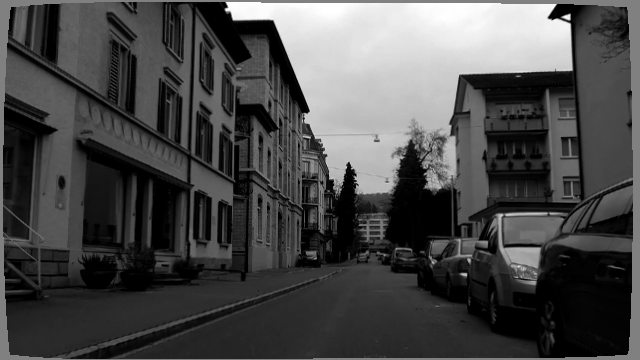
\includegraphics[width=.3\textwidth]{figures/vespa_0014.png}}\hfill
\subfloat[roll while making turns]{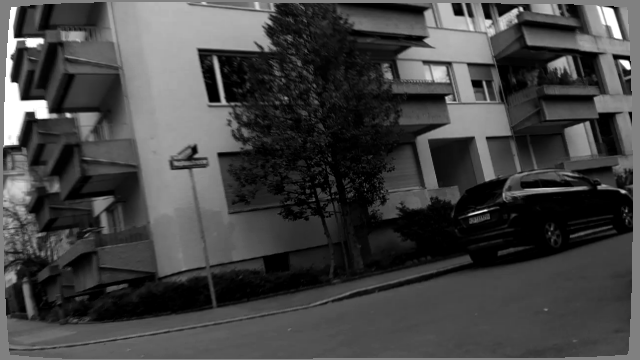
\includegraphics[width=.3\textwidth]{figures/vespa_0292.png}}\hfill
\subfloat[pedestrian traffic]{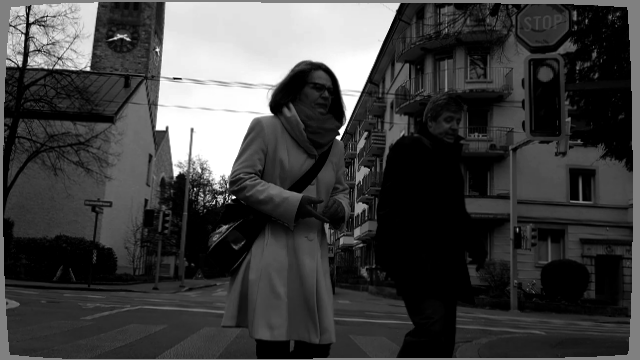
\includegraphics[width=.3\textwidth]{figures/vespa_1072.png}}
\caption{Frames from the \emph{Vespa} data set}
\end{figure}

\section{Bundle Adjustment}
\label{bundle adjustment}
As mentioned in section \ref{additionalWork}, the stand-alone VO pipeline suffers from a significant amount of scale drift. 
This means that along the trajectory, the average scale of the displacements changes due to numerical errors and noise accumulation. 
For continuous operation, a form of overlapping windowed BA was implemented to counteract this drift. \coderef{main.m, runBA.m} 
Every \baEveryNthFrame frames, the trajectory and landmarks are adjusted and replaced over a segment of the last \baReplaceframes frames. 
In order to ensure continuity, the adjusted point cloud and trajectory are constrained such that the last two orientations and locations of the last segment coincide with first two orientations and locations of the newly adjusted segment. \par
In cases where most key points are lost, BA switches to the \emph{Levenberg-Marquardt algorithm}. In these cases the locations and orientations must be aligned manually.

% graphics of BA effect
\begin{figure}[htp]
	\centering
	
	\subfloat[]{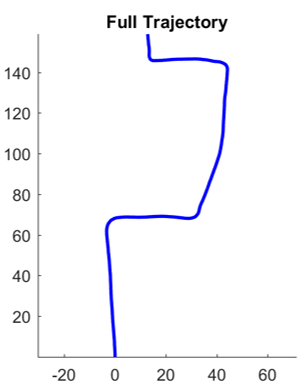
\includegraphics[width=.3\textwidth]{figures/ba_effect.png}}
	\hspace{2cm}
	\subfloat[]{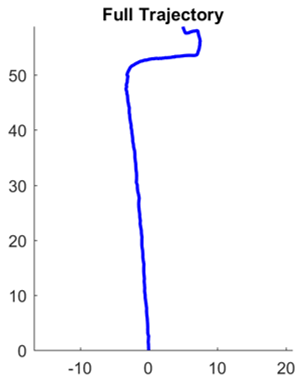
\includegraphics[width=.3\textwidth]{figures/without_ba_effect.png}}
	\caption{Comparison between bundle adjusted trajectory (a) and non-bundle adjusted trajectory (b) over 650 frames in the KITTI dataset with fixed seed rng(1).}
	\label{fig:BAeffect}
\end{figure}


Figure \ref{fig:BAeffect} shows that BA reduces scale drift significantly, smooths the trajectory and maintains the heading more reliably. These advantages come at the price of computing performance: VO with bundle adjustment uses about 40\% more computing time than VO without bundle adjustment.

\section{Ground Truth Alignment and Error Analysis}
\label{simulation}

For a stable operation of the VO pipeline, optimized parameters had to be chosen to control detection and matching of new key points, triangulation etc. 
We determined these parameters by running a simulation \coderef {simMain.m, simTaskScheduler.m} on a benchmark data set (\emph{KITTI}) over various parameter choices. The computed trajectories were aligned with the ground truth and total squared error in orientation (angle deviation) and the total deviation in location was determined for the first 500 frames \coderef{alignToGroundTruth.m}. Using these error metrics, optimal parameters could be identified which will be discussed further in section \ref{performance}. An aligned trajectory can be see in figure \ref{fig:alignment}. This trajectory alignment is done automatically if the flag \emph{align\_to\_ground\_truth} is set.

% graphics of aligned trajectory
\begin{figure}[H]
  \centering
    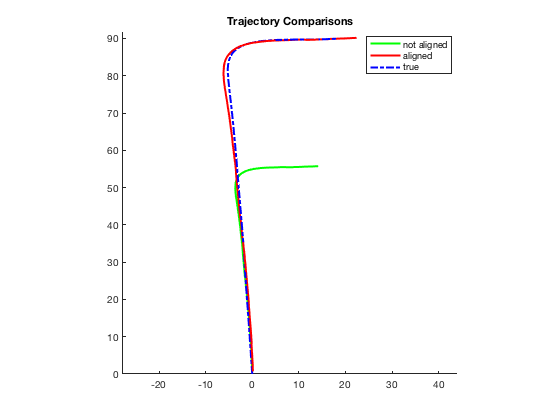
\includegraphics[width=\textwidth]{figures/aligned}
  \caption{Comparison between the non-aligned (green), aligned (red) and true (blue) trajectory. The square deviation of orientation and location between the aligned and true trajectory was chosen as a suitable error metric.}
  \label{fig:alignment}
\end{figure}
% //////